% Wygenerowano przez scal_en.py (skill tlumaczenie-en) z en/main.tex i definicje-en.tex.
% Plik jest NADPISYWANY: poprawki tłumaczenia wprowadzaj w en/*.tex, liczby w skrypcie analizy.
\documentclass[11pt]{article}
\usepackage[utf8]{inputenc}
\usepackage[T1]{fontenc}
\usepackage[english]{babel}
\usepackage[margin=2.5cm]{geometry}
\usepackage{booktabs,graphicx,xcolor,amsmath}
\usepackage[hidelinks]{hyperref}
\usepackage{float}
\usepackage{changepage}
\usepackage{enumitem}
\usepackage{doi}
\usepackage[numbers,sort&compress]{natbib}
\bibliographystyle{plainnat}

\extrafloats{100}
\newcommand{\fillin}[1]{\textcolor{red}{[#1]}}
\RequirePackage{booktabs,csvsimple-l3}
\providecommand{\TabDir}{tabele/}
\providecommand{\FigDir}{rysunki/}
\providecommand{\fillin}[1]{\textbf{[#1]}}
\providecommand{\tabelacsv}[2]{\csvloop{file={\TabDir #2-en.csv}, separator=semicolon, head,
  column names detection=false, after head=\begin{tabular}{#1}\toprule\csvlinetotablerow\\\midrule,
  command=\csvlinetotablerow, late after line=\\, late after last line=\\\bottomrule\end{tabular}}}
\providecommand{\uwagatabeli}[1]{\par\vspace{2pt}\parbox{\linewidth}{\footnotesize #1}}
\newcommand{\DaysOverThreePct}{32.0}
\newcommand{\DaysOverThreeMultiModPct}{84.9}
\newcommand{\DailyQOne}{2}
\newcommand{\DailyQThree}{4}
\newcommand{\NResponses}{57{,}997}
\newcommand{\NEmployees}{180}
\newcommand{\NItems}{164}
\newcommand{\NModules}{9}
\newcommand{\NSequences}{15{,}270}
\newcommand{\NRejected}{0}
\newcommand{\DateStart}{May 2023}
\newcommand{\DateEnd}{June 2026}
\newcommand{\AccOverall}{86.6}
\newcommand{\AccFirst}{82.6}
\newcommand{\AttemptsMedian}{3}
\newcommand{\AttemptsMax}{17}
\newcommand{\SeqRepeatedPct}{78.1}
\newcommand{\SeqMinThreePct}{59.8}
\newcommand{\GapMedian}{37}
\newcommand{\GapQOne}{18}
\newcommand{\GapQThree}{90}
\newcommand{\DailyMedian}{3}
\newcommand{\RespPerEmpMedian}{195}
\newcommand{\RespPerEmpQOne}{70}
\newcommand{\RespPerEmpQThree}{575}
\newcommand{\SpanMonthsMedian}{18}
\newcommand{\ActiveLastQuarterPct}{58.3}
\newcommand{\WeekdayPct}{100.0}
\newcommand{\ItemsPerEmpMedian}{86}
\newcommand{\ActiveDaysMedian}{84}
\newcommand{\OptionsMedian}{3}
\newcommand{\NExcluded}{212}
\newcommand{\NExcludedItems}{2}
\newcommand{\NExcludedItemResp}{348}
\newcommand{\NExcludedShortRep}{88}
\newcommand{\MinGapDays}{7}
\newcommand{\NShortRep}{88}
\newcommand{\NShortRepSameDay}{88}
\newcommand{\ShortRepPct}{0.15}
\newcommand{\NShortRepHour}{80}
\newcommand{\ExcludedModules}{mnk-tst}
\newcommand{\NExcludedPilot}{644}
\newcommand{\NExcludedPilotLater}{2233}
\newcommand{\NExcludedPilotTotal}{2877}
\newcommand{\NPilotSeq}{513}
\newcommand{\NPilotEmp}{72}
\newcommand{\PilotStart}{24 April 2023}
\newcommand{\PilotEnd}{28 April 2023}
\newcommand{\DaysUpToThreePct}{68.0}
\newcommand{\DaysUpToFourPct}{98.8}
\newcommand{\DailyMax}{7}
\newcommand{\HourPOne}{9:05}
\newcommand{\HourPNinetyNine}{15:57}
\newcommand{\HoursNineSixteenPct}{99.3}
\newcommand{\HoursTenFourteenPct}{62.6}
\newcommand{\ReaskAfterCorrect}{73.5}
\newcommand{\ReaskAfterIncorrect}{74.5}
\newcommand{\GapAfterCorrect}{37}
\newcommand{\GapAfterIncorrect}{39}
\newcommand{\AccAttOne}{82.6}
\newcommand{\AccAttOneCI}{[81.1, 84.1]}
\newcommand{\AccAttMax}{92.7}
\newcommand{\AccAttMaxCI}{[90.6, 94.8]}
\newcommand{\AttMax}{10}
\newcommand{\CohortK}{5}
\newcommand{\CohortN}{4890}
\newcommand{\CohortAccOne}{81.9}
\newcommand{\CohortAccK}{89.0}
\newcommand{\CohortAccOneCI}{[79.6, 84.1]}
\newcommand{\CohortAccKCI}{[87.3, 90.7]}
\newcommand{\PowerLawB}{0.29}
\newcommand{\PowerLawRsq}{0.97}
\newcommand{\ORMOneAttempt}{1.39}
\newcommand{\ORMOneAttemptCI}{[1.33, 1.45]}
\newcommand{\PMOneAttempt}{< 0.001}
\newcommand{\ORMTwoAttempt}{1.35}
\newcommand{\ORMTwoAttemptCI}{[1.25, 1.45]}
\newcommand{\PMTwoAttempt}{< 0.001}
\newcommand{\ORMTwoPrev}{3.89}
\newcommand{\ORMTwoPrevCI}{[3.51, 4.31]}
\newcommand{\PMTwoPrev}{< 0.001}
\newcommand{\ORMTwoGap}{0.88}
\newcommand{\ORMTwoGapCI}{[0.86, 0.90]}
\newcommand{\PMTwoGap}{< 0.001}
\newcommand{\ORMTwoTenure}{0.86}
\newcommand{\ORMTwoTenureCI}{[0.76, 0.98]}
\newcommand{\PMTwoTenure}{= 0.020}
\newcommand{\ORMThreeTenure}{0.88}
\newcommand{\ORMThreeTenureCI}{[0.76, 1.01]}
\newcommand{\PMThreeTenure}{= 0.067}
\newcommand{\MOneDropped}{292}
\newcommand{\ICCEmployee}{0.10}
\newcommand{\ICCItem}{0.24}
\newcommand{\SDEmployee}{0.71}
\newcommand{\SDItem}{1.10}
\newcommand{\RsqMarginal}{0.022}
\newcommand{\RsqConditional}{0.36}
\newcommand{\ORRange}{1.29--1.51}
\newcommand{\ORSensMain}{1.39}
\newcommand{\ORSensMainCI}{[1.33, 1.45]}
\newcommand{\ORSensCohort}{1.36}
\newcommand{\ORSensCohortCI}{[1.27, 1.46]}
\newcommand{\ORSensTrunc}{1.39}
\newcommand{\ORSensTruncCI}{[1.33, 1.45]}
\newcommand{\ORSensLenThree}{1.31}
\newcommand{\ORSensLenThreeCI}{[1.22, 1.41]}
\newcommand{\ORSensLenFive}{1.35}
\newcommand{\ORSensLenFiveCI}{[1.26, 1.46]}
\newcommand{\ORSensLenEight}{1.41}
\newcommand{\ORSensLenEightCI}{[1.32, 1.51]}
\newcommand{\ORSensActive}{1.39}
\newcommand{\ORSensActiveCI}{[1.33, 1.46]}
\newcommand{\ORSensTenure}{1.51}
\newcommand{\ORSensTenureCI}{[1.42, 1.61]}
\newcommand{\ORSensGee}{1.29}
\newcommand{\ORSensGeeCI}{[1.24, 1.35]}
\newcommand{\ORSensMixed}{1.38}
\newcommand{\ORSensMixedCI}{[1.34, 1.42]}
\newcommand{\NCorrections}{3382}
\newcommand{\NForgetting}{2719}
\newcommand{\EquilibriumPct}{88.8}
\newcommand{\RetainPct}{92.6}
\newcommand{\RetainCI}{[91.8, 93.4]}
\newcommand{\ForgetPct}{7.4}
\newcommand{\RecoverPct}{58.3}
\newcommand{\RecoverCI}{[55.5, 61.2]}
\newcommand{\PersistPct}{41.7}
\newcommand{\SameDistractorPct}{71.8}
\newcommand{\SameDistractorCI}{[69.4, 74.1]}
\newcommand{\SameDistractorN}{2420}
\newcommand{\SameDistractorExpected}{47.2}
\newcommand{\SameDistractorExpectedPop}{60.0}
\newcommand{\CorrRunOne}{64.4}
\newcommand{\CorrRunOneCI}{[62.2, 66.8]}
\newcommand{\CorrRunTwo}{48.1}
\newcommand{\CorrRunThree}{41.8}
\newcommand{\CorrRunMax}{34.2}
\newcommand{\CorrRunMaxCI}{[27.6, 40.9]}
\newcommand{\CorrRunMaxN}{295}
\newcommand{\RunMax}{4}
\newcommand{\EverCorrectedPct}{81.8}
\newcommand{\FirstWrongSeqN}{2068}
\newcommand{\SameDistrGapShort}{70.6}
\newcommand{\SameDistrGapMid}{73.2}
\newcommand{\SameDistrGapLong}{71.6}
\newcommand{\PersistTopItems}{14}
\newcommand{\PersistTopItemsShare}{39.6}
\newcommand{\PersistItems}{145}
\newcommand{\RetShortCorrect}{95.2}
\newcommand{\RetLongCorrect}{88.5}
\newcommand{\RetShortIncorrect}{60.9}
\newcommand{\RetLongIncorrect}{58.1}
\newcommand{\ForgetShort}{4.8}
\newcommand{\ForgetLong}{11.5}
\newcommand{\ForgetRunOne}{11.9}
\newcommand{\ForgetRunOneCI}{[10.7, 13.0]}
\newcommand{\ForgetRunTwo}{7.6}
\newcommand{\ForgetRunThree}{5.0}
\newcommand{\ForgetRunMax}{3.2}
\newcommand{\ForgetRunMaxCI}{[2.7, 3.7]}
\newcommand{\ForgetFreshShort}{7.7}
\newcommand{\ForgetFreshLong}{13.9}
\newcommand{\ForgetStableShort}{2.3}
\newcommand{\ForgetStableLong}{5.2}
\newcommand{\RelapsePct}{24.9}
\newcommand{\RelapseCI}{[22.9, 26.8]}
\newcommand{\RelapseN}{2457}
\newcommand{\RelapseSamePct}{73.6}
\newcommand{\RelapseSameCI}{[69.5, 77.7]}
\newcommand{\RelapseSameN}{611}
\newcommand{\ForgetRunK}{4}
\newcommand{\EmpN}{148}
\newcommand{\EmpImproved}{101}
\newcommand{\EmpWorsened}{18}
\newcommand{\EmpUnchanged}{29}
\newcommand{\EmpMeanChange}{4.1}
\newcommand{\EmpMeanChangeCI}{[2.7, 5.5]}
\newcommand{\SignP}{< 0.001}
\newcommand{\WilcoxonP}{< 0.001}
\newcommand{\RankBiserial}{0.77}
\newcommand{\EmpSharePct}{82.2}
\newcommand{\ItemDifficultyMedian}{85.5}
\newcommand{\TopDistractorMedian}{71.9}
\newcommand{\NDistractors}{349}
\newcommand{\NNonFunctional}{196}
\newcommand{\NonFunctionalPct}{56.2}
\newcommand{\ItemsModerate}{102}
\newcommand{\ItemsGoodDisc}{50}
\newcommand{\ItemsDiscTested}{161}
\newcommand{\ItemsImproving}{43}
\newcommand{\ItemsWorsening}{1}
\newcommand{\ItemsTestable}{164}
\newcommand{\ItemDiscMedian}{0.23}
\newcommand{\ItemsLowDisc}{65}
\newcommand{\ItemsEasy}{58}
\newcommand{\ItemsHard}{4}
\newcommand{\TopItems}{10}
\newcommand{\DemoN}{180}
\newcommand{\DemoMatched}{151}
\newcommand{\DemoMatchedPct}{83.9}
\newcommand{\DemoUnmatched}{29}
\newcommand{\DemoWomen}{121}
\newcommand{\DemoWomenPct}{80.1}
\newcommand{\DemoMen}{30}
\newcommand{\DemoMenPct}{19.9}
\newcommand{\DemoSexMissing}{29}
\newcommand{\DemoAgeN}{150}
\newcommand{\DemoAgeMissing}{30}
\newcommand{\AgeMedian}{47}
\newcommand{\AgeQOne}{41}
\newcommand{\AgeQThree}{56}
\newcommand{\AgeMin}{22}
\newcommand{\AgeMax}{67}
\newcommand{\AgeMean}{47.2}
\newcommand{\AgeSD}{10.6}
\newcommand{\AgeModalGroup}{50--59}
\newcommand{\AgeModalGroupPct}{34.0}
\newcommand{\FirstN}{15{,}270}
\newcommand{\FirstAcc}{82.6}
\newcommand{\FirstAccCI}{[81.2, 84.1]}
\newcommand{\FirstAccMinGroup}{30--39}
\newcommand{\FirstAccMin}{74.9}
\newcommand{\FirstAccMaxGroup}{50--59}
\newcommand{\FirstAccMax}{84.3}
\newcommand{\FirstAgeOR}{1.16}
\newcommand{\FirstAgeORCI}{[1.03, 1.31]}
\newcommand{\FirstAgeP}{= 0.012}
\newcommand{\FirstAgeN}{13{,}578}
\newcommand{\FirstAgeEmp}{150}
\newcommand{\FirstAgeRawOR}{1.12}
\newcommand{\FirstAgeRawORCI}{[1.01, 1.24]}
\newcommand{\FirstAgeRawP}{= 0.039}
\newcommand{\SeqChange}{7.2}
\newcommand{\SeqChangeCI}{[5.5, 8.9]}
\newcommand{\SeqChangeMinGroup}{60--69}
\newcommand{\SeqChangeMin}{4.0}
\newcommand{\SeqChangeMaxGroup}{40--49}
\newcommand{\SeqChangeMax}{8.8}
\newcommand{\SeqAgeOR}{0.97}
\newcommand{\SeqAgeORCI}{[0.90, 1.05]}
\newcommand{\SeqAgeP}{= 0.484}
\newcommand{\SeqAgeN}{23{,}140}
\newcommand{\BootReps}{2000}
\newcommand{\Alpha}{0.05}
\newcommand{\MinItemN}{30}
\newcommand{\Seed}{2026}
\newcommand{\MaxAttemptPooled}{10}
\newcommand{\VerPython}{3.14.4}
\newcommand{\VerPandas}{3.0.3}
\newcommand{\VerNumpy}{2.5.0}
\newcommand{\VerScipy}{1.18.0}
\newcommand{\VerStatsmodels}{0.14.6}
\newcommand{\VerMatplotlib}{3.11.0}

\usepackage{authblk}
\renewcommand\Authand{ and }\renewcommand\Authands{, and }
\author[1,*]{Bartosz Lewandowski \small{(ORCID:0009-0004-1158-0693)}}
\author[2]{Monika Szerszeń \small{(ORCID: 0009-0009-6625-3979)}}
\author[3]{Magdalena Dowgalec \small{(ORCID:0009-0005-4469-2832)}}
\author[4]{Ewaryst Tkacz \small{(ORCID:0000-0003-2580-7954)}}
\author[5]{Maciej J. Wróbel \small{(ORCID:0000-0003-1865-2122)}}

\affil[1,4]{Department of Clinical Engineering, Academy of Silesia, Katowice, Poland}
\affil[2]{Banking Process Support and Optimization Department, Powiślański Cooperative Bank, Kwidzyn, Poland}
\affil[3]{Legal Department, Atende SA, Warsaw, Poland}
\affil[5]{Department of Otolaryngology and Oncological Laryngology, Collegium Medicum NCU, Toruń, Poland}

\affil[*]{Corresponding author: Bartosz Lewandowski, bartosz.lewandowski@akademiaslaska.pl}

\title{Employee response accuracy on repeated questions: forgetting and persistent errors in a three-year microlearning program}

\date{}
\begin{document}
\maketitle

\begin{abstract}
\noindent\textbf{Background.} Spaced repetition improves retention, but the effectiveness of
microlearning in organizations has rarely been assessed using multi-year data on employee responses.
\textbf{Methods.} The analysis covered \NResponses{} responses from \NEmployees{} bank employees to
\NItems{} multiple-choice questions, given from \DateStart{} to \DateEnd. Questions recurred on
a schedule independent of response outcome (median interval \GapMedian{} days), and the correct answer
with an explanation was displayed after every response. Accuracy was analyzed across successive
attempts at the same question and by the outcome of, and interval since, the previous attempt.
\textbf{Results.} Accuracy at the first attempt was \FirstAcc\%. In sequences of at least
\CohortK{} attempts, it rose from \CohortAccOne\% to \CohortAccK\% (by \SeqChange{} pp, 95\% CI
\SeqChangeCI). Error corrections outnumbered forgetting events (\NCorrections{} vs.\
\NForgetting).
The forgetting rate increased with the interval and decreased with the number of consecutive correct
responses, from \ForgetRunOne\% after one to \ForgetRunMax\% after at least \ForgetRunK{}. In
\SameDistractorPct\% of cases, repeated errors involved the same distractor (expected under choice
proportional to distractor popularity: \SameDistractorExpectedPop\%), regardless of the interval.
\textbf{Conclusions.} Accuracy on recurring questions increased, but knowledge required further
repetition, and some errors persisted despite feedback. A schedule adapted to employee performance and
feedback addressing the selected distractor may increase the effectiveness of such programs.

\medskip\noindent\textbf{Keywords:} spaced repetition; microlearning; employee training; feedback;
forgetting; learning analytics
\end{abstract}

\section{Introduction}

Retrieving information from memory strengthens it more than rereading does (the testing effect), and
learning distributed over time is more durable than massed learning (the spacing effect)
\citep{roediger2006,cepeda2006}. Both effects are combined in spaced education, in which short
multiple-choice questions recur periodically over weeks or months. In studies involving physicians and
other health professionals, it improved the acquisition and retention of knowledge
\citep{kerfoot2009,phillips2019}.

In organizations, a similar format is used in \emph{microlearning}, that is, short training units,
often in the form of quizzes. Evidence of its effectiveness, however, comes mainly from studies with
small samples and from grey literature \citep{taylor2022}, and the effects of mandatory employee
training, e.g., in information security, tend to be small or to fade over time
\citep{reinheimer2020}. Training effectiveness is usually assessed through transfer, that is, the
application of knowledge at work \citep{blume2010}. Transfer, however, requires that the knowledge
first be acquired and retained.

This earlier stage can be examined using data from microlearning platforms. The platform records each
response together with its time and outcome, and the same question returns to the same employee
repeatedly. Successive responses are therefore repeated measurements of the same knowledge in the same
person. Similar data are used in learner models applied in intelligent tutoring systems and language
learning applications \citep{corbett1994,settles2016}.

The study was conducted in a bank in which employees answered short questions displayed on their
computers during the working day, and the system collected the responses over three years. Questions
recurred on a schedule independent of response outcome, and the correct answer was displayed after
every response. Such a schedule makes it possible to compare error corrections and forgetting without
the selection introduced by adaptive algorithms, which is rare in data from training platforms.
Laboratory studies further indicate that a selected distractor can become fixed in memory and that
errors made with high confidence can recur despite feedback \citep{butler2008,butler2011}. Whether this
phenomenon occurs in employee training is not known. Three research questions were formulated:
(RQ1) does the percentage of correct responses increase when the same question returns to the same
employee;
(RQ2) how does accuracy depend on the outcome of the previous attempt and on the time elapsed since it;
(RQ3) do repeated errors persist despite feedback, which would point to misconceptions rather than to
guessing.
\section{Materials and methods}

\subsection{Training program}
The study was conducted in a bank. The questions were prepared by the \textit{Banking Process Support
and Optimization Department}, which also decided on employee participation in the program. The
questions concerned knowledge used in everyday work at the bank. Each was a multiple-choice question
with three to five answer options, one of which was correct, while the others were
\emph{distractors}. The questions, answer options and explanations were written in Polish.

The training application started automatically on working days on employees' computers and displayed
one to four randomly selected questions per day, between 9:00 and 16:00. After each response, correct
or incorrect, it showed the correct answer with an explanation (\emph{feedback}). The same question
could return to an employee no earlier than after seven days, and the repetition schedule did not
depend on the response outcome. The program was suspended while the questions were reviewed and
updated. In the analyzed data, the median number of responses per employee on an active day was
\DailyMedian{} (IQR \DailyQOne--\DailyQThree). The same question returned after a median of
\GapMedian{} days (IQR \GapQOne--\GapQThree).

An example question presented to program participants, on cybersecurity, read:
``Which of the following situations is phishing?''. Answer options:
``1 - A DDoS attack'',
``2 - Installing antivirus software'',
``3 - Backing up data'',
``4 - A fake e-mail with a link to the bank's login page (marked as the correct answer)''.
Explanation displayed after the response:
``Phishing is a fraud method in which someone impersonates a trusted person or institution (e.g., a bank, a courier, a public office) to trick you into revealing confidential data such as passwords, card numbers or logins. Most often it looks like an e-mail from the `bank' with an urgent request to log in, a text message with a link to an `extra payment for a parcel', or a fake website deceptively similar to the real one. The key mechanism is that the fraudster creates a sense of urgency or stress so that you click without thinking. IMPORTANT: do not click suspicious links, always check the website address (URL), do not enter your login details via a link from a message, and if something looks `too urgent', it is often a scam.''.

\subsection{Data and study population}
\label{sec:dane}
The recorded employee responses were analyzed. Each record contained the question, the selected
option, the employee code, the date and time of the response, and whether the response was correct.
The analytical dataset comprised \NResponses{} responses
(Table~\ref{tab:zbior_danych}). The bank also provided a summary of employees' age and sex.

\begin{table}[H]
\centering
\caption{Characteristics of the dataset.}
\label{tab:zbior_danych}
\small
\begin{tabular}{lr}
\toprule
Characteristic & Value \\
\midrule
Responses & 57{,}997 \\
Employees & 180 \\
Questions & 164 \\
Observation period & 2023-05-10 -- 2026-06-08 \\
Employee--question sequences & 15{,}270 \\
Observed answer options per question, median (range) & 3 (2--5) \\
\midrule
Responses per employee, median [IQR] & 195 [70, 575] \\
Questions per employee, median [IQR] & 86 [38, 138] \\
Active days per employee, median [IQR] & 84 [30, 224] \\
Responses per active day, median [IQR] & 3 [2, 4] \\
Months between first and last response, median [IQR] & 18 [5, 30] \\
\midrule
Attempts per sequence, median [IQR] (max.) & 3 [2, 5] (17) \\
Sequences with $\geq$2 / $\geq$3 attempts (\%) & 78.1 / 59.8 \\
Days between attempts, median [IQR] & 37 [18, 90] \\
\midrule
Correct responses, overall (\%) & 86.6 \\
Correct responses, first attempts (\%) & 82.6 \\
\bottomrule
\end{tabular}
\uwagatabeli{IQR: interquartile range. A sequence is a series of attempts by one employee at one
question. The number of observed answer options may be smaller than the number of options in the
question because some options were not chosen by any employee. Excluded test responses: \NExcluded.
Excluded questions with a single observed answer option: \NExcludedItems{} (\NExcludedItemResp{}
responses). Excluded repetitions given earlier than \MinGapDays{} days after the previous attempt:
\NExcludedShortRep.}
\end{table}

Demographic data were available for \DemoMatched{} of the \DemoN{} employees (\DemoMatchedPct\%).
Women accounted for \DemoWomenPct\% of persons of known sex ($n = \DemoWomen$). The median age was
\AgeMedian{} years (IQR \AgeQOne--\AgeQThree; range \AgeMin--\AgeMax), and the largest age group was
\AgeModalGroup{} years (\AgeModalGroupPct\%; Table~\ref{tab:demografia}). Age was included in the
analysis of the first attempt and of the rate of accuracy gain; sex was not analyzed.

\begin{table}[H]
\centering
\caption{Demographic characteristics of the employees included in the analysis.}
\label{tab:demografia}
\small
\begin{tabular}{lr}
\toprule
Characteristic & Value \\
\midrule
Employees included in the analysis & 180 \\
of whom with demographic data, $n$ (\%) & 151 (83.9) \\
\midrule
Women, $n$ (\%) & 121 (80.1) \\
Men, $n$ (\%) & 30 (19.9) \\
Sex not recorded, $n$ & 29 \\
\midrule
Age (years), median [IQR] & 47 [41, 56] \\
Age (years), mean (SD) & 47.2 (10.6) \\
Age (years), range & 22--67 \\
\midrule
20--29 years, $n$ (\%) & 13 (8.7) \\
30--39 years, $n$ (\%) & 21 (14.0) \\
40--49 years, $n$ (\%) & 49 (32.7) \\
50--59 years, $n$ (\%) & 51 (34.0) \\
60--69 years, $n$ (\%) & 16 (10.7) \\
Age not recorded, $n$ & 30 \\
\bottomrule
\end{tabular}
\uwagatabeli{Percentages by sex were calculated among persons of known sex, and percentages by age
group among persons of known age ($n = \DemoAgeN$). Missing data concern mainly employees absent from
the demographic summary (\DemoUnmatched). IQR: interquartile range; SD: standard deviation.}
\end{table}

In the response database, employees were identified by a random code, and the demographic summary was
linked to the recorded responses using this code. Such a code cannot be reconstructed from a list of
employees; the analyzed data were therefore fully anonymized.

\subsection{Statistical analysis}
\label{sec:analiza}
The responses of one employee to one question, ordered in time, formed a \emph{sequence}. The position
of a response in the sequence was termed the \emph{attempt number}, and the first response, that is,
the employee's first encounter with the question, the \emph{first attempt}. The \emph{interval} was the
number of days since the previous attempt in the same sequence, and \emph{accuracy} was the percentage
of correct responses. Accuracy was reported with 95\% confidence intervals (CI) obtained with the
bootstrap: employees were resampled with replacement (\BootReps{} replicates), which accounts for the
dependence between responses given by the same person. In regression models, standard errors were
clustered by employee.

\emph{First attempt.} Accuracy at the first attempt was compared across age groups. The association
with age (10-year groups) was estimated by logistic regression with question fixed effects, that is,
with a separate intercept for each question. Question difficulty was not recorded in the data, so the
fixed effects were estimated from the responses of all employees. The model thus compared employees of
different ages answering the same questions. For comparison, it was also fitted without question fixed
effects.

\emph{Changes within a sequence (RQ1).} Accuracy was calculated for successive attempt numbers;
attempts \MaxAttemptPooled{} and later were pooled. With each attempt, the number of sequences
decreased, and employees who continued responding could differ from the others, which distorts
aggregate curves \citep{murray2013}. The change was therefore also assessed in a \emph{cohort}, that
is, in sequences of at least \CohortK{} attempts, restricted to attempts 1 to \CohortK{}. Accuracy at
each of these attempts was calculated for the same sequences, and the measure of change was the
difference between attempt~\CohortK{} and attempt~1 in percentage points (pp).
The association between the rate of gain and age was tested in the cohort by logistic regression with
an interaction between $\log_2$ attempt number and age, and with employee and question fixed effects.

\emph{Outcome of the previous attempt and interval (RQ2).} Each attempt from the second onward was
assigned to one of four categories according to the outcome of that attempt and of the previous one:
a correct response after a correct one, \emph{error correction} (correct after incorrect),
\emph{forgetting} (incorrect after correct) or \emph{repeated error} (incorrect after incorrect).
Because the error-correction rate ($r$) and the forgetting rate ($f$) have different denominators, the
numbers of both events were compared, and the equilibrium level $r/(r+f)$, toward which accuracy would
tend at constant rates, was determined. The rates were compared across six interval bins:
\MinGapDays--13, 14--29, 30--59, 60--119, 120--239 and at least 240 days. The forgetting rate was also
tabulated by the number of consecutive correct responses before a given attempt and separately after an
error correction. An incorrect response at the attempt following an error correction was termed an
\emph{error relapse}, and it was checked whether the employee chose the same distractor as before the
correction. It was also checked whether the repetition schedule depended on the outcome of the
previous attempt.

\emph{Persistent errors (RQ3).} Accuracy was compared by the number of \emph{consecutive errors}, that
is, successive incorrect responses immediately preceding a given attempt, from 0 to at least \RunMax.
For two successive errors, the frequency with which the employee chose the same distractor was
calculated and compared with the percentage expected under random choice and under choice
proportional to distractor popularity in the given question. This percentage was also tabulated in
three interval bins: shorter than 30 days, 30--89 days and at least 90 days. The share of repeated
errors concentrated in the 10\% of questions with the most such errors was also calculated.

Computations were performed in Python \VerPython{} using pandas \VerPandas, NumPy \VerNumpy, SciPy
\VerScipy, statsmodels \VerStatsmodels{} and Matplotlib \VerMatplotlib.
\section{Results}

\subsection{First attempt}
At the first encounter with a question (\FirstN{} responses from \NEmployees{} employees), accuracy
was \FirstAcc\% (95\% CI \FirstAccCI; Table~\ref{tab:pierwsza_proba_wiek}). Accuracy varied with age
non-monotonically: it was lowest in the \FirstAccMinGroup{} age group (\FirstAccMin\%) and highest in
the \FirstAccMaxGroup{} age group (\FirstAccMax\%). When responses to the same questions were
compared, the odds of a correct response increased with age (OR \FirstAgeOR{} per 10 years, 95\% CI
\FirstAgeORCI; $p \FirstAgeP$). Without question fixed effects, the association was weaker
(OR \FirstAgeRawOR, 95\% CI \FirstAgeRawORCI; $p \FirstAgeRawP$).

\begin{table}[H]
\centering
\caption{Accuracy at the first attempt, overall and by employee age group.}
\label{tab:pierwsza_proba_wiek}
\footnotesize
\setlength{\tabcolsep}{4pt}
\begin{tabular}{l*{7}{r}}
\toprule
Age group (years) & Overall & 20--29 & 30--39 & 40--49 & 50--59 & 60--69 & Missing \\
\midrule
Employees & 180 & 13 & 21 & 49 & 51 & 16 & 30 \\
First attempts, $n$ & 15{,}270 & 970 & 2011 & 4338 & 5096 & 1416 & 1439 \\
Accuracy (\%) & 82.6 & 82.5 & 74.9 & 84.0 & 84.3 & 82.6 & 83.5 \\
95\% CI & [81.2, 84.1] & [77.5, 89.3] & [68.8, 80.7] & [81.5, 86.3] & [82.2, 86.5] & [78.7, 86.4] & [80.0, 86.8] \\
\bottomrule
\end{tabular}%
\uwagatabeli{The first attempt is the first response in a sequence. 95\% CIs were obtained with the
bootstrap. The association with age was estimated by the logistic regression described in
Section~\ref{sec:analiza} (\FirstAgeN{} responses from \FirstAgeEmp{} employees of known age):
OR \FirstAgeOR{} per 10 years, 95\% CI \FirstAgeORCI, $p \FirstAgeP$.}
\end{table}

\subsection{Changes within a sequence (RQ1)}
Accuracy increased with attempt number, from \AccAttOne\% \AccAttOneCI{} at the first attempt to
\AccAttMax\% \AccAttMaxCI{} at attempt \AttMax{} and later (Figure~\ref{fig:krzywa_uczenia}). Because
the number of sequences decreased with each attempt, the change was examined in a cohort of
\CohortN{} sequences. In the cohort, accuracy rose from \CohortAccOne\% \CohortAccOneCI{} at
attempt~1 to \CohortAccK\% \CohortAccKCI{} at attempt~\CohortK{}, that is, by \SeqChange{} pp
(95\% CI \SeqChangeCI; Table~\ref{tab:sekwencje_wiek}). An increase within the same sequences means
that the improvement did not result from the earlier termination of sequences with lower accuracy.
Accuracy at attempt~1 in the cohort (\CohortAccOne\%) was close to accuracy at the first attempt in
all sequences (\FirstAcc\%).

The estimated increase was positive in all age groups and ranged from \SeqChangeMin{} pp
(\SeqChangeMinGroup{} years) to \SeqChangeMax{} pp (\SeqChangeMaxGroup{} years), although in the small
extreme age groups the lower limit of the 95\% CI was close to zero. The rate of increase did not
depend on age (interaction OR \SeqAgeOR{} per 10 years of age and doubling of attempt number, 95\% CI
\SeqAgeORCI; $p \SeqAgeP$).

\begin{figure}[H]
\centering
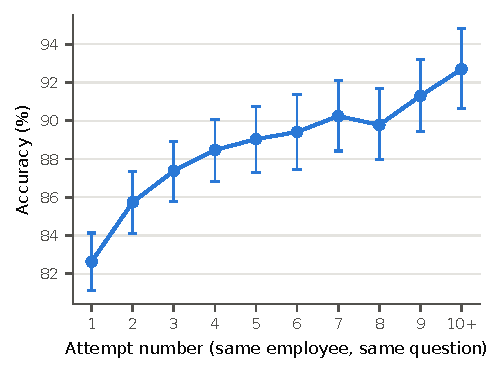
\includegraphics{rysunki/rys_krzywa_uczenia-en}
\caption{Accuracy by attempt number in all sequences available at a given attempt (their number
decreases with attempt number). Error bars: 95\% CI (bootstrap). Attempts \MaxAttemptPooled{} and
later were pooled. The course in the cohort is shown in Figure~\ref{fig:stany_kohorty}.}
\label{fig:krzywa_uczenia}
\end{figure}

\begin{table}[H]
\centering
\caption{Accuracy at successive attempts in the cohort, overall and by employee age group.}
\label{tab:sekwencje_wiek}
\footnotesize
\setlength{\tabcolsep}{4pt}
\begin{tabular}{l*{7}{r}}
\toprule
Age group (years) & Overall & 20--29 & 30--39 & 40--49 & 50--59 & 60--69 & Missing \\
\midrule
Employees & 124 & 9 & 15 & 35 & 39 & 13 & 13 \\
Sequences, $n$ & 4890 & 199 & 664 & 1784 & 1689 & 471 & 83 \\
\midrule
Attempt 1 (\%) & 81.9 & 81.4 & 77.0 & 81.6 & 83.8 & 82.4 & 86.7 \\
Attempt 2 (\%) & 85.6 & 80.4 & 79.4 & 85.7 & 88.0 & 86.6 & 94.0 \\
Attempt 3 (\%) & 87.2 & 85.4 & 81.5 & 88.5 & 88.3 & 86.0 & 95.2 \\
Attempt 4 (\%) & 88.4 & 87.9 & 82.7 & 89.5 & 89.7 & 86.2 & 96.4 \\
Attempt 5 (\%) & 89.0 & 86.9 & 84.2 & 90.4 & 90.1 & 86.4 & 97.6 \\
\midrule
Change, attempt 5 vs 1 (pp) & 7.2 & 5.5 & 7.2 & 8.8 & 6.3 & 4.0 & 10.8 \\
95\% CI & [5.5, 8.9] & [0.0, 14.7] & [3.2, 13.5] & [5.9, 11.6] & [4.3, 8.1] & [0.0, 9.3] & [1.9, 19.8] \\
\bottomrule
\end{tabular}%
\uwagatabeli{Cohort: sequences of at least \CohortK{} attempts, attempts 1 to \CohortK{}.
pp: percentage points; 95\% CIs of the change were obtained with the bootstrap. The association between
the rate of improvement and age was estimated by the logistic regression described in
Section~\ref{sec:analiza} (\SeqAgeN{} responses from employees of known age).}
\end{table}

\subsection{Outcome of the previous attempt and interval (RQ2)}
The increase in accuracy results from two opposing processes: error correction and forgetting. The
schedule did not bias their comparison, because a question returned after a correct and after an
incorrect response with similar probability (\ReaskAfterCorrect\% and \ReaskAfterIncorrect\%) and
after a similar interval (median \GapAfterCorrect{} and \GapAfterIncorrect{} days). After a correct
response, the next one was correct in \RetainPct\% \RetainCI{} of cases, and forgetting occurred in
\ForgetPct\%. After an incorrect response, an error correction followed in \RecoverPct\%
\RecoverCI{} of cases. These rates refer to different groups of attempts, so the numbers of events were
also compared: there were \NCorrections{} error corrections and \NForgetting{} forgetting events. The
predominance of corrections explains the increase in accuracy. At constant error-correction and
forgetting rates, accuracy would tend toward an equilibrium level of \EquilibriumPct\%. Accuracy in the
cohort at attempt~\CohortK{} (\CohortAccK\%) was close to this level, but at attempts \AttMax{} and
later it was \AccAttMax\% and exceeded it. This is because the forgetting rate was not constant but
depended on the interval and on the number of consecutive correct responses.

The forgetting rate increased with the interval, from \ForgetShort\% at intervals shorter than 14 days
to \ForgetLong\% at intervals of at least 240 days (Figure~\ref{fig:odstep}). The error-correction
rate changed less with the interval (\RetShortIncorrect\% and \RetLongIncorrect\% in the same bins).

The forgetting rate also depended on the number of consecutive correct responses. After one correct
response, it was \ForgetRunOne\% \ForgetRunOneCI, after two \ForgetRunTwo\%, after three
\ForgetRunThree\%, and after at least \ForgetRunK{} \ForgetRunMax\% \ForgetRunMaxCI{}
(Table~\ref{tab:seria_poprawnych}). The difference persisted at every interval: at intervals shorter
than 14 days, the forgetting rate was \ForgetFreshShort\% after one and \ForgetStableShort\% after at
least three correct responses, and at intervals of at least 240 days \ForgetFreshLong\% and
\ForgetStableLong\%, respectively. Error corrections were the least durable. After a correction, an
error relapse occurred in \RelapsePct\% \RelapseCI{} of cases ($n = \RelapseN$), and in
\RelapseSamePct\% \RelapseSameCI{} of these the employee chose the same distractor as before the
correction. This share was similar to the percentage of repeated choices of the same distractor after
two successive errors (\SameDistractorPct\%; Section~\ref{sec:pb3}).

\begin{figure}[H]
\centering
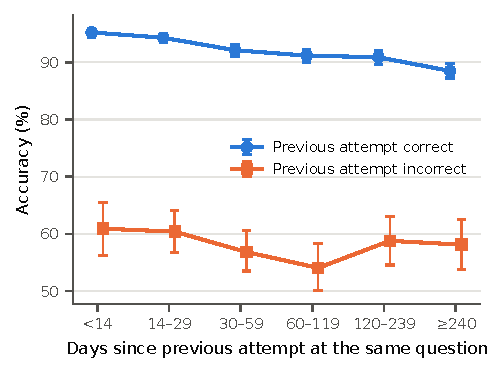
\includegraphics{rysunki/rys_odstep-en}
\caption{Accuracy by interval, separately for attempts preceded by a correct response (circles) and by
an incorrect response (squares). For attempts preceded by a correct response, the forgetting rate is
100\% minus accuracy; for attempts preceded by an incorrect response, accuracy is the error-correction
rate. Error bars: 95\% CI (bootstrap).}
\label{fig:odstep}
\end{figure}

\begin{table}[H]
\centering
\caption{Forgetting rate by the number of consecutive correct responses given immediately before
a given attempt.}
\label{tab:seria_poprawnych}
\footnotesize
\setlength{\tabcolsep}{5pt}
\begin{tabular}{l*{4}{r}}
\toprule
Consecutive correct before attempt & 1 & 2 & 3 & $\geq$4 \\
\midrule
Attempts, $n$ & 12{,}318 & 8276 & 5597 & 10{,}734 \\
Employees & 159 & 147 & 137 & 123 \\
Forgetting rate (\%) & 11.9 & 7.6 & 5.0 & 3.2 \\
95\% CI & [10.7, 13.0] & [6.7, 8.5] & [4.2, 5.8] & [2.7, 3.7] \\
\bottomrule
\end{tabular}%
\uwagatabeli{Attempts preceded by a correct response. Forgetting rate: percentage of incorrect
responses. 95\% CIs were obtained with the bootstrap.}
\end{table}

\subsection{Persistent errors (RQ3)}
\label{sec:pb3}
Most errors were corrected: in \EverCorrectedPct\% of the \FirstWrongSeqN{} sequences that began with
an incorrect response and comprised at least two attempts, the employee later answered correctly at
least once. The chance of correction, however, decreased with each successive error. After one error,
accuracy was \CorrRunOne\% \CorrRunOneCI, after two consecutive errors \CorrRunTwo\%, after three
\CorrRunThree\%, and after at least \RunMax{} \CorrRunMax\% \CorrRunMaxCI{}
(Table~\ref{tab:seria_bledow}). Part of this decrease may be due to several consecutive errors
occurring mainly in more difficult questions.

Repeated errors were not consistent with random choice. After two successive errors, the employee
chose the same distractor in \SameDistractorPct\% \SameDistractorCI{} of cases
($n = \SameDistractorN$), whereas \SameDistractorExpected\% would be expected under random choice and
\SameDistractorExpectedPop\% under choice proportional to distractor popularity. This percentage did
not depend on the interval (\SameDistrGapShort\% at intervals shorter than 30 days,
\SameDistrGapMid\% at 30--89 days and \SameDistrGapLong\% at intervals of at least 90 days). Repeated errors were
concentrated in few questions: \PersistTopItems{} of the \PersistItems{} questions accounted for
\PersistTopItemsShare\% of them.

\begin{table}[H]
\centering
\caption{Accuracy by the number of consecutive errors made immediately before a given attempt.}
\label{tab:seria_bledow}
\footnotesize
\setlength{\tabcolsep}{5pt}
\begin{tabular}{l*{5}{r}}
\toprule
Consecutive errors before attempt & 0 & 1 & 2 & 3 & $\geq$4 \\
\midrule
Attempts, $n$ & 36{,}925 & 4024 & 1074 & 409 & 295 \\
Employees & 159 & 149 & 110 & 80 & 48 \\
Accuracy (\%) & 92.6 & 64.4 & 48.1 & 41.8 & 34.2 \\
95\% CI & [91.9, 93.4] & [62.2, 66.8] & [44.7, 51.9] & [36.4, 47.3] & [27.6, 40.9] \\
\bottomrule
\end{tabular}%
\uwagatabeli{Attempts from the second onward. Column 0: attempts preceded by a correct response.
95\% CIs were obtained with the bootstrap.}
\end{table}

\subsection{Summary of results}
Figure~\ref{fig:stany_kohorty} summarizes the results in the cohort. Accuracy increases from attempt
to attempt (RQ1), error corrections outnumber forgetting events (RQ2), and at every attempt from the
second onward, part of the incorrect responses are repeated errors (RQ3).

\begin{figure}[H]
\centering
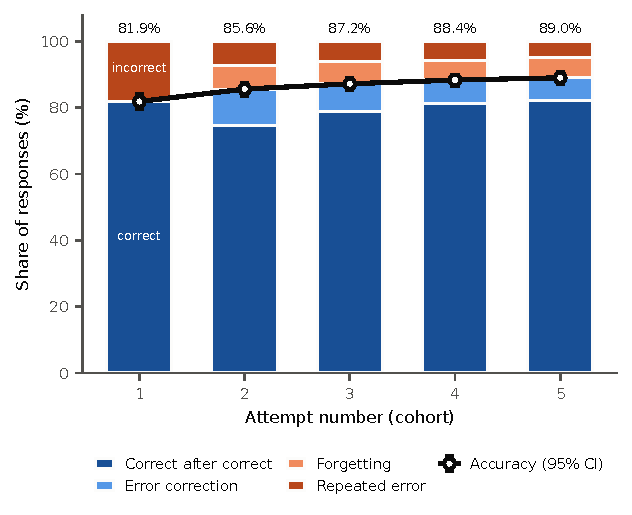
\includegraphics{rysunki/rys_stany_kohorty-en}
\caption{Accuracy and response state in the cohort (\CohortN{} sequences, attempts 1 to \CohortK{}).
Bars: share of responses by the outcome of the current and the previous attempt
(Section~\ref{sec:analiza}); at attempt~1, only correct and incorrect responses. Line: accuracy with
95\% CI (bootstrap), values above the bars.}
\label{fig:stany_kohorty}
\end{figure}
\section{Discussion}

In the bank's microlearning program, response accuracy increased with each return of a question, also
in the cohort in which the same sequences were compared. The increase resulted from error corrections
outnumbering forgetting events. Some errors, however, persisted despite feedback and consisted in
choosing the same distractor again.
The direction of change is consistent with studies of spaced education in medical training.
In urology residents, the knowledge advantage gained from periodically recurring questions persisted
two years after the end of the program \citep{kerfoot2009}, and a systematic review of studies on
clinicians' continuing professional development indicated a beneficial effect of this method on the
acquisition and retention of knowledge \citep{phillips2019}.

The conditions of those studies, however, differed from those of the present analysis. The
participants were health professionals, and the effect was usually assessed with a test administered
outside the program, in comparison with a control group. In the program studied here, the participants
were bank employees, and the increase in accuracy was observed only in responses given within the
program itself. The agreement therefore concerns the direction of change, not the size of the effect or
its cause. The results do, however, show what the increase in accuracy consisted of, which a final test
score does not reveal. It was the difference between two opposing processes, error correction and
forgetting (\NCorrections{} vs.\ \NForgetting{} events), and the same overall increase could also
arise with more frequent forgetting if it were accompanied by a correspondingly larger number of
corrections. Aggregate measures also do not detect errors that persist despite feedback.

Forgetting was associated with three factors. The first was the passage of time: forgetting was more
frequent at longer intervals, in line with research on the spacing between repetitions
\citep{cepeda2006}. The second was a short history of correct responses. Knowledge confirmed by one
correct response was forgotten two to four times more often than knowledge confirmed several times in
a row, at every interval.
Similarly, in studies of repeated practice, each additional successful retrieval increased the
durability of knowledge \citep{rawson2013}. The third factor was error relapse. Error correction proved
the least durable, and when it did not hold, the employee usually returned to the distractor chosen
before the correction. The return of original errors after feedback has also been described in
laboratory studies \citep{butler2011}. The correct answer may thus not have replaced the misconception
but coexisted with it.

Repeated errors differed in character from forgetting. Employees chose the same distractor more often
than chance would predict, regardless of the interval, and each successive error reduced the chance of
correction. Such a pattern is consistent with a persistent misconception rather than with a lack of
knowledge, which would lead to guessing. A selected distractor can become fixed in memory, and feedback
reduces this effect \citep{butler2008}. In the program studied, the feedback gave the correct answer
and an explanation but did not address the selected distractor, although explaining why the selected
answer is wrong is usually more effective \citep{shute2008}. The concentration of repeated errors in
\PersistTopItems{} questions further suggests that some of them resulted from question design, e.g.,
an ambiguous distractor or content inconsistent with the bank's practice. Such questions can be
identified by standard distractor analysis \citep{gierl2017}.

In one-off training, e.g., in information security, the effects faded after several months
\citep{reinheimer2020}. The present results indicate that knowledge requires further repetition also in
a program with periodically recurring questions, and that the way these repetitions are scheduled can
be improved. Because the interval did not depend on the outcome, mastered questions returned as often
as questions in which the employee had only just corrected an error. An adaptive schedule could
lengthen the interval after several consecutive correct responses and shorten it after an error
correction, when the risk of relapse is highest. Personalized review improved long-term retention
compared with a fixed schedule \citep{lindsey2014}, and models of forgetting rate based on response
history are already used in language learning applications \citep{settles2016}. A second change could
be feedback addressing the selected distractor, introduced first in the questions with the largest
number of repeated errors.

\subsection{Limitations and future research}
The study was observational and had no control group, so the increase in accuracy cannot be attributed
solely to the program, as employees also acquired knowledge in their everyday work. Because the
questions were repeated, the data do not allow consolidation of knowledge to be distinguished from
memorization of the answer to a specific question. Response time and employee confidence were not
recorded, so forgetting cannot be separated from inattention or from a lucky guess at an earlier
attempt, which learner models capture as slip and guess \citep{corbett1994}. Such a source of part of
the forgetting is suggested by its rate of \ForgetShort\% already at intervals shorter than 14 days.
The longest intervals may have included periods when the program was suspended, so changes in question
content may have inflated the forgetting rate at these intervals. The comparisons were descriptive and
were not corrected for multiple testing. The confidence intervals accounted for the dependence between
responses of the same employee, but not of the same question. The associations with the number of
consecutive correct responses or errors may therefore partly reflect differences in difficulty between
questions.

Future studies could compare, in a randomized design, a fixed with an adaptive schedule and standard
feedback with feedback addressing the selected distractor, using equivalent versions of questions that
would separate knowledge from memorization of the answer. Recording response confidence would make it
possible to test whether persistent errors concern high-confidence beliefs \citep{butler2011}.
Microlearning outcomes should also be linked to the application of knowledge at work, e.g., to the
number of procedural errors \citep{blume2010}.

\section{Conclusions}
In a program with periodically recurring questions, the response accuracy of bank employees increased
from attempt to attempt. Knowledge nevertheless required further repetition, because it was forgotten
over time, particularly after the first correct response and after an error correction. Some errors
persisted despite feedback and consisted in choosing the same distractor again. A schedule adapted to
employee performance and feedback addressing the selected distractor may increase the effectiveness of
such programs, but their effect requires confirmation in studies with a control group.

\section*{Declarations}

\noindent\textbf{Ethics.}
The study used fully anonymized data provided by the bank with its written consent of 3 August 2026.
Employee coding and data protection rules are described in Section~\ref{sec:dane}.\\
\textbf{Data availability.}
The data used in the study are the property of the bank and are not publicly available.\\
\textbf{Funding.}
The study received no funding.\\
\textbf{Competing interests.}
M. Szerszeń is an employee of the bank in which the study was conducted. The other authors declare no
competing interests.\\
\textbf{Use of AI tools.}
During the preparation of this article, the authors used Anthropic Claude Sonnet 5.5 for (1) language
editing of the description of the results of the analysis performed by the authors and (2) translation
of the text from Polish into English. Data analysis, interpretation of the results and conclusions were
carried out by the author. The authors verified and edited the entire text and take full responsibility
for its content.

\bibliography{references}
\end{document}
